\documentclass[12pt,a4paper]{article}
\usepackage[utf8]{inputenc}
\usepackage[russian]{babel}
\usepackage[OT1]{fontenc}
\usepackage{mathtools}
\usepackage{amsfonts}
\usepackage{amssymb}
\usepackage{enumitem}
\usepackage{alltt}
\usepackage{graphicx}
\usepackage{indentfirst}
\usepackage{caption}
\usepackage{float}
\usepackage{wrapfig}
\setlength{\parindent}{0.75cm}
\graphicspath{{pictures/}}
\DeclareGraphicsExtensions{.png}
\usepackage[left=15mm,right=15mm,top=2cm,bottom=2cm]{geometry}
\author{Глотов Алексей}
\begin{document}
\newpage
\begin{center}
\footnotesize{{ГОСУДАРСТВЕННОЕ АВТОНОМНОЕ ОБРАЗОВАТЕЛЬНОЕ УЧРЕЖДЕНИЕ}\break
{ВЫСШЕГО ОБРАЗОВАНИЯ}
\break
{\bf {МОСКОВСКИЙ ФИЗИКО-ТЕХНИЧЕСКИЙ ИНСТИТУТ}}
\break
\small{(НАЦИОНАЛЬНЫЙ ИССЛЕДОВАТЕЛЬСКИЙ УНИВЕРСИТЕТ)}}
\break
\hfill \break
\hfill \break
\begin{center}
\normalsize{Кафедра общей физики}
\end{center}
\hfill \break
\hfill \break
\hfill \break
\hfill \break

\begin{center}
\normalsize {Лабораторная работа 1.3.1-1.3.2}
\end{center}
\hfill \break\\
\large{Определение модуля Юнга тонкой проволоки посредством ее растяжения, определение модуля кручения с помощбю крутильного матника}
\end{center}
\begin{flushleft}
\hfill \break
\hfill \break
\hfill \break
\hfill \break
\hfill \break
\hfill \break
\hfill \break
\hfill \break
\hfill \break
\hfill \break
\hangindent=9cm
\normalsize{Преподаватель:}\hfill
\normalsize{к.ф.-м.н., доц. Яворский В.А.}\\
\hfill \break
\normalsize{Обучающийся:}\hfill
\normalsize{Глотов А.А} \\
\hfill \break
\end{flushleft}
\hfill \break
\hfill \break
\hfill \break
\hfill \break
\hfill \break
\hfill \break
\hfill \break
\hfill \break
\hfill \break
\hfill \break
\hfill \break

\begin{center}
Долгопрудный \break
 2021
\end{center}
\thispagestyle{empty}
\newpage
\begin{center}
\large{\bf Введение} 
\end{center}
\begin{center}
\large{Цели работы} \break
\end{center}
\begin{itemize}
\item Эксперементальная проверка зависимости между напряжением и деформацией (Закон Гука) для одноосного растяжения
\item Получение модюля Юнга для тонкой проволоки
\item Исследование зависимости углов закручивания в зависимости от приложенного момента сил для крутильного маятника
\item Рассчет модуля кручения и сдвига для крутильного маятника по измерениям периода куртильных колебаний
\end{itemize}
\hfill \break
\begin{center}
\large{Приборы и материалы}
\end{center}
\begin{enumerate}
\item Прибор Лермонтова
\item Проволока из исследуемого материала
\item Зрительная трубка со шкалой
\item Набор грузов
\item Микрометр
\item Рулетка
\item Секундомер
\item Линейка
\end{enumerate}
\newpage
\begin{center}
\large{Теоретические сведения} \break
{Часть 1}
\end{center}
\hfill \break
\begin{par}
{Примем за ось Х ось, в направлении которой растягивается наша проволока,тогда справделива будет формула}
\end{par}
\begin{center}
${\sigma=E\varepsilon}$ (1)
\end{center} 
{Тогда при отстутствии $F_{y}$ и $F_{z}$ справедливо}
\begin{center}
\large $\frac{\Delta{l_{x}}}{{l_{x}}}=\frac{\sigma_{x}}{E}$ (2)
\end{center}
Или
\begin{center}
$F=k\Delta{x}$  \;\;\;\;\;\;\; $k=\frac{ES}{l_{x}}$ (3)
\end{center}
{Измерения проводятся на следующей установке}
\begin{center}
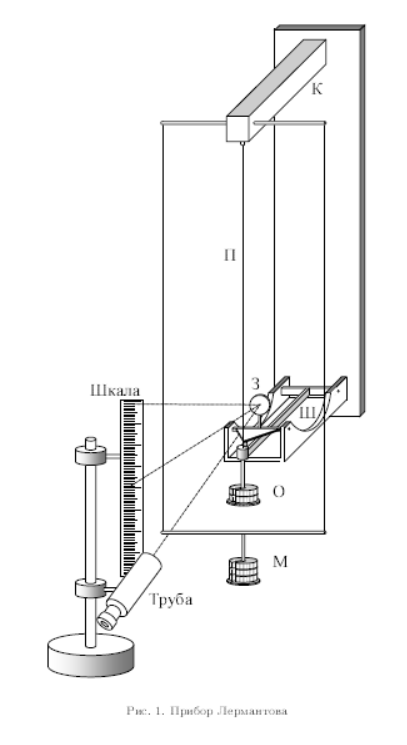
\includegraphics{1.3.1_2} \break
\end{center}
\begin{par}
Отметим, что т.к. проволока изначально не в идеальном состоянии, необходимо приложить некоторую силу, чтобы убрать изначальные деформации. Поэтому начальные точки с большой вероятностью не лягут на прямую
\end{par} 
\begin{par}
Необходимо учесть, что проволока имеет свое разрушающее напряжение, при достижении которого уже не возвращается в исходное состояние. Поэтому необходимо проводить измерения в пределах 30 процентов от разрушаещего напряжения, которое определяется серией экспериментов 
\end{par}
\begin{par}
Определим связь между удлинением проволоки и значением шкалы, снимаемым с помощью трубки. Очевидно, что при малых удлинениях угол $\alpha$ мал, и тогда
\end{par}
\begin{center}
\large $\tan(\alpha)=\alpha=\frac{\Delta{l}}{r}$ (4)
\end{center}
В то же время направление луча изменится на $2\alpha$, причем d в малых изменениях справедливо
\begin{center}
\large $2\alpha=\frac{x}{h}$ \;\;\;\;\;\;\; $x=\frac{nL}{N}$ (5)
\end{center}
$\frac{L}{N}$ - длина одного деления шкалы
\hfill \break
\hfill \break
Приравнивая (4) к (5) получим 
\begin{center}
\large $\Delta{l}=\frac{nrL}{2Nh}$ (6)
\end{center}
\begin{center}
\hfill \break
Часть 2
\break
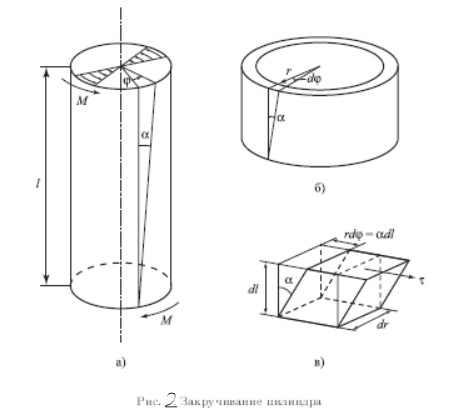
\includegraphics{1.3.1_1} \break
\end{center}
\par {Рассмотрим часть закручиваемого круглого цилиндра (см.рис 2a)}{Рассмотрим кольцо радиуса r с бесконечно малой толщиной dr и бесконечно малой высотой dl. При небольшом угле скручивания выполняется}
\begin{center}
\large $\alpha{dl}=rd\varphi$ (7)
\end{center}
{Касательное напряжение $\tau$ связано с углом сдвига и модулем сдвига G соотношением}
\begin{center}
\large $\tau=G\alpha$ (8)
\end{center}
{Подставляя (7) в (8) получим}
\begin{center}
\large $\tau=Gr\frac{d\varphi}{dl}$ (9)
\end{center}
{Касательные напряжения создают момент сил относительно оси цилиндра}
\begin{center}
\large $dM=2\pi{rdr}\cdot{\tau}\cdot{r}$ (10)
\end{center}
{Суммарный момент цилиндра определим как интеграл по радиусу}
\begin{center}
\large $M=2\pi{G}\frac{d\varphi}{dl}\int_0^R r^3\,\mathrm{d}r=\pi{G}\frac{d\varphi}{dl}\frac{R^4}{2}$ (11)
\end{center}
{Момент неизменен по длине и линейно зависит от угла поворота. Тогда для цилиндра M определяется как}
\begin{center}
\large $M=\frac{\pi{R^4G}}{2l}\varphi=f\varphi$ \;\;\;\;\;\;\; $f=\frac{\pi{R^4}G}{2l}$(12)
\end{center}
{f - модуль кручения}
{Вращение вокруг вертикальной оси под действием упругого момента, возникающего в проволоке описывается уравнением}
\begin{center}
\large $I\frac{d^2\varphi}{dt^2}=-M$ (13)
\end{center}
{I - момент инерции вращаемого тела, $\varphi$ - угол поворота от положения равновесия, M - момент упругих сил. При малых колебаниях M описывается по формуле}
\begin{center}
\large $M=\frac{\pi{R^4G}}{2l}\varphi$ (14)
\end{center}
{Введем}
\begin{center}
\large $\omega^2=\frac{f}{I}$(15)
\end{center}
{Получаем уравнение гармонических колебаний}
\begin{center}
\large $\frac{d^2\varphi}{dt^2}+\omega^2\varphi=0$
\end{center}
{Его решение имеет вид}
\begin{center}
\large $\varphi=\varphi_{0}\sin(\omega{t}+\theta)$ \;\;\;\;\;\;\; $T=2\pi{\sqrt{\frac{I}{f}}}$ (16)
\end{center}
\begin{par}
{Отметим, что полученные уравнения справедливы только для идеальных (незатухающих) колебаний. Поэтому необходимо убедиться, что затуханием можно пренебречь. Это будет выполняться, если после 10 колебаний амплитуда уменьшается менее чем в 2 раза, а период не зависит от начальной амплитуды}
\end{par}
\newpage
\begin{center}
\large {\bf Ход работы}\break
Часть 1
\end{center}
1)\large \;\; Определение сечения проволоки 
\par
Диаметр проволоки примем известным (определен и фисирован для установки)\hfill \break
$<d>= 0,46\text{мм} \;\;\;\;\; \Delta{d} = 0.01\text{мм}$ 
\hfill \break
2) Измерение длины проволоки
\hfill \break
\hfill \break
$l_{0}=176.0\text{см}$ \;\;\;\;\;\;\;\;\;\;\;\;\;\;\;\;\;\;\; $\sigma^{instr}_{l_{0}}=0.2\text{см}$
\hfill \break
\hfill \break
3) Возьмем необходимую зависимость из теоретической части (6)
\hfill \break
\large $\frac{L}{N}=1\text{мм}$
\par Тогда $x = \frac{L}{N}n$, причем х в мм численно равен n
\hfill \break
4) Отметим, что имеющихся грузов (общей массой 2208,5г недостаточно для достижения 30 процентов от разрушающего напряжения. Зная диаметр проволоки, нетрудно посчитать, что для этого необходима масса примерно 5кг. По мере выполнения п.5 убедимся, что проволока действительно возвращается в исходное состояние 
\hfill \break
\hfill \break
5)\;Снимем зависимость n(m)
\hfill \break
\hfill \break
\begin{tabular}{|c|c||c|c||c|c||c|c|}
\hline 
x, мм & m, г & x, мм & m, г & x, мм & m, г & x, мм & m, г \\ 
\hline 
0 & 0 & -221 & -2208,5 & 0 & 0 & -221 & -2208,5 \\ 
\hline 
29 & 245,6 & -195 & -1962,9 & 23 & 245,6 & -194 & -1962,9 \\ 
\hline 
55 & 490,9 & -167 & -1718,5 & 52 & 490,9 & -165 & -1718,5 \\ 
\hline 
78 & 736,2 & -143 & -1473,3 & 77 & 736,2 & -140 & -1473,3 \\ 
\hline 
103 & 982,3 & -118 & -1227,8 & 102 & 982,3 & -115 & -1227,8 \\ 
\hline 
128 & 1227,8 & -94 & -982,3 & 126 & 1227,8 & -92 & -982,3 \\ 
\hline 
152 & 1473,3 & -71 & -736,2 & 150 & 1473,3 & -68 & -736,2 \\ 
\hline 
175 & 1718,5 & -48 & -490,9 & 174 & 1718,5 & -44 & -490,9 \\ 
\hline 
200 & 1962,9 & -23 & -245,6 & 197 & 1962,9 & -21 & -245,6 \\ 
\hline 
223 & 2208,5 & 0 & 0 & 218 & 2208,5 & 0 & 0 \\ 
\hline 
\end{tabular} 
\hfill \break 
\hfill \break
$\Delta{n}=1 \;\;\;\;\; \sigma_{x} = 1 \text{мм}$
\hfill \break
6)
\begin{center}
$F=\frac{ES}{l_{x}}l=\frac{E\pi{d^2}}{4l_{x}}l$ 
\end{center}
Пересчитаем x в l по (6)\hfill \break
$r=13.0 \text{см} \;\;\;\; h=135.0 \text{см} \;\;\;\; l_{0}=176\text{см}$
\flushleft $\sigma_{r}= 0.1 \text{см} \;\;\;\;\;\;\;\; \sigma_{h}=0.2 \text{см} \;\;\;\;\;\;\; \sigma_{l_{0}}=0.2\text{cм}$ \hfill \break
Отметим, что $\frac{\sigma_{h}}{h}$ примерно в 5 раз меньше $\frac{\sigma_{r}}{r}$ Тогда $\varepsilon_{l}=\varepsilon_{r}=0.8\%$
\begin{tabular}{|c|c|c|c|c|c|c|c|}
\hline 
l, см & m, г & l, см &  m, г &l, см & m, г &l, см & m, г \\ 
\hline 
0 & 0 & 0,106 & 2208,5 & 0 & 0 & 0,106 & 2208,5 \\ 
\hline 
0,014 & 245,6 & 0,094 & 1962,9 & 0,011 & 245,6 & 0,093 & 1962,9 \\ 
\hline 
0,026 & 490,9 & 0,080 & 1718,5 & 0,025 & 490,9 & 0,079 & 1718,5 \\ 
\hline 
0,038 & 736,2 & 0,069 & 1473,3 & 0,037 & 736,2 & 0,067 & 1473,3 \\ 
\hline 
0,050 & 982,3 & 0,057 & 1227,8 & 0,049 & 982,3 & 0,055 & 1227,8 \\ 
\hline 
0,062 & 1227,8 & 0,045 & 982,3 & 0,061 & 1227,8 & 0,044 & 982,3 \\ 
\hline 
0,073 & 1473,3 & 0,034 & 736,2 & 0,072 & 1473,3 & 0,033 & 736,2 \\ 
\hline 
0,084 & 1718,5 & 0,023 & 490,9 & 0,084 & 1718,5 & 0,021 & 490,9 \\ 
\hline 
0,096 & 1962,9 & 0,011 & 245,6 & 0,095 & 1962,9 & 0,010 & 245,6 \\ 
\hline 
0,107 & 2208,5 & 0 & 0 & 0,105 & 2208,5 & 0 & 0 \\ 
\hline 
\end{tabular} 
\hfill \break	
\hfill \break
По данным таблицы построим график (см. график 1) зависимости l(m)
\begin{center}
$l=m\frac{4gl_{0}}{\pi{Ed^2}}=m\frac{g}{k}$ 
\end{center}
\begin{figure}[h]
\centering
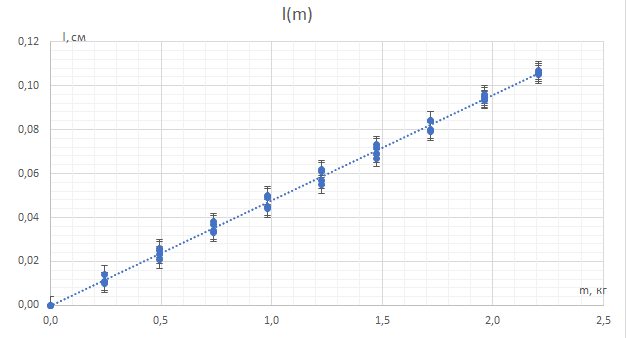
\includegraphics[width=18cm, height=10cm]{1.3.1_gr_1}
\caption{График 1}
\label{gr:1}
\end{figure}
Обозначим коэффицент наклона графика за $\alpha$ \break
Методом наименьших квадратов определим значение и погрешность $\alpha$. Прямая должна идти через 0. Тогда \hfill \break
$\alpha=\frac{<lm>}{<m^2>}=4.8*10^{-4}\frac{\text{м}}{\text{кг}}$ \hfill \break \hfill \break
$\sigma^{\text{случ}}_{\alpha}=\sqrt{\frac{1}{39}(\frac{<{l}^2>}{<m^2>}-{\alpha}^2)}=7.1*10^{-6}\frac{\text{м}}{\text{кг}}$ \;\;\;\;\; \hfill \break
$\frac{\sigma^{\text{случ}}_{\alpha}}{\alpha}=\frac{\sigma^{\text{случ}}_{E}}{E}=\frac{\sigma^{\text{случ}}_{k}}{k}$ \hfill \break
\hfill \break
$\sigma^{\text{приб}}_{k}=k\sqrt{(\frac{\Delta{l}}{l})^2+(\frac{\Delta{m}}{<m>})^2+(\frac{\Delta{g}}{g})^2}=k\varepsilon_{l}$ \hfill \break
$\sigma^{\text{приб}}_{E}=E\sqrt{(\frac{l_{0}}{l_{0}})^2+(\frac{\Delta{l}}{l})^2+4(\frac{\Delta{d}}{d})^2+(\frac{\Delta{g}}{g})^2}=E\varepsilon_{l}$ \hfill \break
При подсчете приборных погрешностей мы пренебрегли всеми погрешнотями, кроме l, ввиду их относительной малости \hfill \break 
Полная погрешность k и E выразится как \hfill \break
$\sigma_{k}=\sqrt{(\sigma^{\text{случ}}_{k})^2+(\sigma^{{\text{приб}}}_{k})^2}$ \hfill \break
$\sigma_{E}=\sqrt{(\sigma^{\text{случ}}_{E})^2+(\sigma^{{\text{приб}}}_{E})^2}$ \hfill \break
Тогда определим значения и погрешности значений k и E \hfill \break
$k=2.05*10^{4}\frac{H}{\text{м}} \;\;\;\;\; E=2.16*10^{11}\frac{H}{\text{м}^2}$ \hfill \break 
$\sigma_{k}=0.4*10^{3}\frac{H}{\text{м}} \;\;\;\;\; \sigma_{E}=0.4*10^{10}\frac{H}{\text{м}^2}$ \hfill \break 
$\varepsilon_{k}=2.0\% \;\;\;\;\; \varepsilon_{E}=1.9\%$ \hfill\break
8) По табличным данным получаем, что наши результаты с наиболшей точностью удовлетворяют характеристикам стали(модуль Юнга лежит в диапазоне $(21,2-22,0)*10^{10}) \text{Па}$
\newpage
\begin{center}
Часть 2
\end{center}
1) Измеряя периоды 10 колебаний для случайного угла амплитуды и примерно в два раза меньшего получим времена колебаний $t=34.3c$ и $t=34.2c$ при приборной погрешности $\Delta{t}=0.3c$. Тогда можно говорить, что в пределах погрешности это одно и то же время. Отметим измеряемую амплитуду, и все дальнейшие измерения будем проводить, устанавливая амплитуду не более отмеченной и будем считать такие колебания малыми.\hfill \break
2) Установим амплитуду колебаний такую же, как в первом пункте. Замерим 10 колебаний и в момент прохождения точек остановки (точки максимального отклонения от точки равновесия) последнего колебания, отметим эти положения. Сравнив их с исходным, получим, что они отличие точно меньше двухкратного. Значит, колебания в пределах установленной амплитуды при 10 колебаниях колебания можно считать слабозатухающими. Значит, возможно использование формул для идеальных колебаний (формулы 7-16).
$\Delta_{T}=\Delta_{t}/10$ \;\;\;\;\; $\Delta_{l} = 1 \text{мм}$
С учетом округления $\Delta_{t} = 0.1 c$
\hfill \break
3) Проведем измерения крутильных колебаний для различных l - расстояний от точки подвеса до грузов \hfill \break
\begin{center}
\begin{tabular}{|c|c|c|c|c|}
\hline 
l, \text{мм} & t, c & T, c & $l^2$, $\text{м}^2*10^{-3}$ & $T^2$, $c^2$ \\ 
\hline 
154 & 44.6 & 4.5 & 23.72 & 19.9 \\ 
\hline 
142 & 42.0 & 4.2 & 20.16 & 17.6 \\ 
\hline 
133 & 39.1 & 3.9 & 17.69 & 15.3 \\ 
\hline 
122 & 36.8 & 3.7 & 14.88 & 13.5 \\ 
\hline 
112 & 33.9 & 3.4 & 12.54 & 11.5 \\ 
\hline 
103 & 31.3 & 3.1 & 10.61 & 9.8 \\ 
\hline 
92 & 28.7 & 2.9 & 8.46 & 8.2 \\ 
\hline 
83 & 26.2 & 2.6 & 6.89 & 6.9 \\ 
\hline 
45 & 17.5 & 1.8 & 2.03 & 3.1 \\ 
\hline 
\end{tabular} 
\end{center}
$I_{\text{гр}}$ - Момент инерции для одного груза \break
Используем закон Гюйгенса-Штейнера и подставим все в (16). Тогда
\begin{center}
$T^2=\frac{4\pi^2}{f}(2m(\frac{I_{\text{гр}}}{m}+l^2)+I_{st})$
\end{center}
$I_{st}$ - момент инерции стержня(ось движения цилиндров)
\begin{figure}[H]
\centering
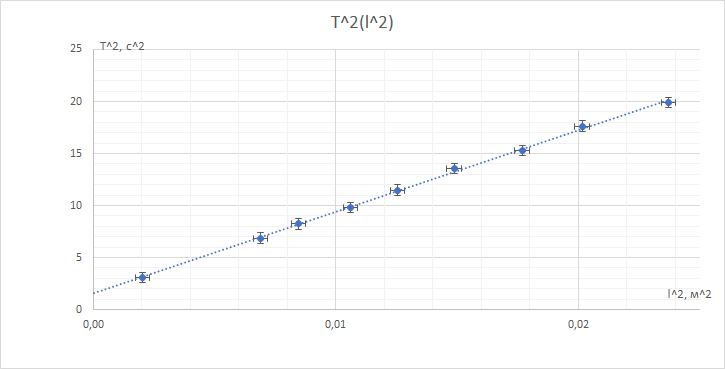
\includegraphics[width=18cm, height=10cm]{1.3.1_gr_2}
\caption{График 2}
\label{gr:1}
\end{figure}
\hfill \break
Обозначим угловой коэффициент прямой за $\beta$
\begin{center}
$\beta=\frac{8\pi^2m}{f}=\frac{256\pi{ml_{0}}}{d^4G}$
\end{center}
$\beta=\frac{<T^2l^2>-<T^2><l^2>}{<l^4>-<l^2>^2}=785.5\frac{c^2}{\text{м}^2}$ \hfill \break
$\sigma^{\text{случ}}_{\beta}=\sqrt{\frac{1}{7}(\frac{<T^4>-<T^2>^2}{<l^4>-<l^2>^2}-\beta^2)}=10,6\frac{c^2}{\text{м}^2}$ \hfill \break
$\frac{\sigma^{\text{случ}}_{\beta}}{\beta}=\frac{\sigma^{\text{случ}}_{G}}{G}$ \hfill \break
4) $l_{0}$ - длина проволоки \break
d - диаметр проволоки \break
m - масса одного цилиндра \break
$l_{0}=1.75\text{м} \;\;\;\;\; \sigma_{l_{0}}=0.02\text{м}$  \break
$d=1.98\text{мм} \;\;\;\;\; \sigma_{d}=0.01\text{мм}$ \break
$m = 373.5\text{г} \;\;\;\;\; \sigma_{m} = 0.3\text{г}$ \break
5) $G=\frac{32fl}{\pi{d^4}}$ \hfill \break
Тогда приборную погрешность G рассчитаем по следующей формуле:
$\sigma^{\text{приб}}_{G}=G\sqrt{(\frac{\Delta{l}}{l})^2+16(\frac{\Delta{d}}{d})^2}$\break
$\sigma_{G}=\sqrt{(\sigma^{\text{приб}}_{G})^2+(\sigma^{\text{случ}}_{G})^2}$ \hfill \break
6) Получим итоговое значение G \break
$G=4.4*10^{10}\frac{H}{\text{м}^2} \;\;\;\;\; \sigma_{G}=0.1*10^{10}\frac{H}{\text{м}^2}$\hfill \break
$\varepsilon_{G}=2.7\%$
\newpage
\begin{center}
Выводы
\end{center}
\par
\;\;\;\;\;{При измермениях растижения проволоки и периода крутильных основная вклад в погрешность вносит погрешность проведения прямой, на ее фоне погрешности измерений необходимых величин являются пренебрежимо малыми. Значит, улучшением точности измерений добиться значительного улучшения точности итоговых данных добиться невозможно, для этого потребуется изменение метода измерений.}
\par 
\;\;\;\;\;{Значения E и G  были получены с точностью 1,7\% и 2.7\%. Это говорит о том, что методы получения значений являются достоточно точными.}
\par 
\;\;\;\;\;{Значение E лежит на интервале $(21.2-22.0)*10^{10}\frac{H}{\text{м}^2}$. Наиболее точно это значение удовлетворяет значению модуля Юнга стали$(20-21)*10^{10})\frac{H}{\text{м}^2}$, однако проволока также могла быть и медной (20,4$\frac{H}{\text{м}^2}$)}
\par 
\;\;\;\;\;{Значение G ледит на интервале $(4.3-4.5)*10^{10}\frac{H}{\text{м}^2}$. Эти значения удовлетворяют возможным значений модуля сдвига для меди (3,5-4,9), что позволяет с высокой точностью утверждать, что материал, из которого изговолена проволока - медь. Однако в вероятный интервал полученного значения модуля сдвига также попадает титан (4,38), что делает его вероятным материалом изготовления проволоки.}
\end{document}